\chapter{Thread Domains}

In an application like ACE there are many subsystems. A lot of calls from
one subsystem to another are pure notifications without results. For instance
the collaboration layer does not want to slow down the logic server of the
session when one connection to a participant is slow. Therefore it is
often desirable to decouple the caller from the receiver by executing calls
on other threads.

That is where the idea of thread domains started. Instead of manually coding
the code to execute a method on another thread we decided to create a general
approach that works universally with objects implementing arbitrary interfaces.



\section{Introduction}

\subsection{Requirements}
There were several requirements that existed when designing the thread
domain concept.

\begin{itemize}
 \item asynchronous method invocations (invoke and forget)
 \item general applicability
 \item flexible thread creation, reuse of threads
 \item keep code testable in presence of potential multithreading
\end{itemize}

The most important requirement was to invoke methods asynchronously. 
The caller of methods with a void return type often do not want to wait
for the end of the execution. For instance if the collaboration layer wants
to send a request to a participant it does not want to wait for the end
of the transmission, because that may be a potentially slow operation. 
Further, if the collaboration layer would wait until each message is sent,
it would slow down the whole processing of other requests, which is highly
undesirable.

It would be easy to achieve the asynchronous method invocation requirement
with custom code. One naive solution consists in simply implementing the target
interface by creating and starting a thread which then does the method
invocation.

\small{\begin{verbatim}
 public class ServiceImpl implements Service {
   protected Service target;
   public void doService(String message) {
     new Thread() {
       public void run() {
         target.doService(message);
       }
     }.start();
   }
 }
\end{verbatim}}

Implementing this pattern whenever an asynchronous invocation is desired
is tedious at best. Beside the obvious problem of starting a new thread
each time a method is invoked, which could be remedied by the use of
a thread pool, it is still less than ideal, because it needs custom code
to invoke the target method. Further, this has nothing to do with the
target objects logic. In AOP (aspect oriented programming) parlance this
is clearly a cross-cutting concern. Invoking methods asynchronously can 
be applied to any object, no matter how it is implemented. It is therefore
required that the implemented solution is generally applicable.

Placing thread creation code in a lot of different places in an application
makes it difficult to manage and tune the usage of threads (see for instance
the code example above). Thread domains should help to control the
number and reuse of threads in an application.

One drawback of introducing multithreading in a codebase is loss of
testability. As soon as there are multiple threads in a system, it is
hard to achieve deterministic tests, thus resulting in a less testable
system. Therefore, thread domains should help to introduce multithreading
without sacrificing testability.


\subsection{Idea}
The idea of a thread domain is to create a dynamic proxy which stands
in for a real target object. The dynamic proxy is responsible that the
invocation is invoked in another \emph{threading domain}. So what is
a threading domain? A threading domain is a part of an application
which is executed by a set of designated worker threads. The set may
contain just one thread in which case the code inside that thread domain
does not have to do any special synchronizations.

A thread domain provides a way to wrap an existing object with the dynamic
proxy object, which in turn takes care that the invocations to the
target object are carried out inside the thread domain (i.e. by one of
the workers of the thread domain).

The programmer has to take care that all incoming references
to a particular subsystem are properly wrapped if it is the purpose to
make sure that only one thread (or the thread domain's set of threads)
executes code in the subsystem. If thread domains are simply used to
invoke methods asynchronously such measures have not to be taken. The
concept is still applicable and useful.


\subsection{Basic Design}
\label{sect:threaddomain.introduction.principle}
Figure \ref{fig:threaddomain_basic} shows the principle of thread domains.
The first object involved is a proxy, which is responsible to
capture all the necessary information so that the method invocation can
be executed at a later point. This includes the target object, the method
to be invoked, as well as all the method parameters. This proxy then adds
the method invocation to a queue. After these few steps the proxy returns
to the caller. As there is no return value available from the method 
invocation (the real method has not been invoked yet), the proxy returns
the null for objects, zero, or false depending on the return type of the
invoked method.

A worker thread is waiting on the blocking queue for method invocations.
Whenever a method invocation is available that method invocation object
is removed from the queue and executed on the worker thread.

\begin{figure}[H]
 \centering
 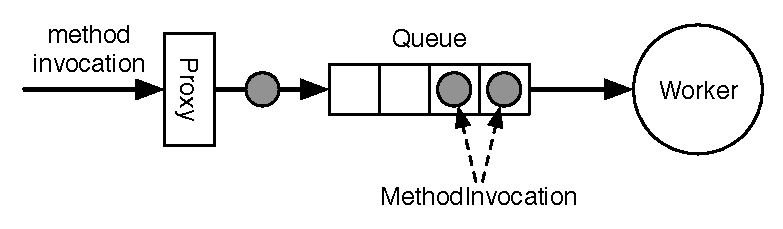
\includegraphics[width=13cm,height=3.4cm]{../images/finalreport/threaddomain_basic.eps}
 \caption{Basic Thread Domain Architecture}
 \label{fig:threaddomain_basic}
\end{figure}



\section{Implementation}

\subsection{ThreadDomain Interface}
The core interface is \texttt{ch.iserver.ace.util.ThreadDomain}.
The most important methods exposed by that interface are the \texttt{wrap}
methods. These methods allow to wrap an object so that all method invocations
to that object are executed in that thread domain. This interface is the only 
interface users of thread domains need to know.

The basic principle was already described earlier 
(see \ref{sect:threaddomain.introduction.principle}). However the exact
implementation of thread domains can vary significantly. The most significant
differences are found in the management of worker threads.


\subsection{Proxy Implementation}
One of the requirements was that thread domains should work universally across
different classes. This is achieved by using the facilities provided by
Java 1.3, namely dynamic proxies. Although the implementation does not use
these dynamic proxies directly, it uses them through the Spring AOP facilities.

The code to \emph{wrap} an object in a thread domain can be found in the
abstract base class \texttt{ch.iserver.ace.util.AbstractThreadDomain}. The
core classes used in the protected \texttt{wrap} methods are the
\texttt{org.springfactory.aop.framework.ProxyFactory} class and the 
\texttt{org.aopalliance.intercept.MethodInterceptor}. 

The proxy implementation is found in 
\texttt{ch.iserver.ace.util.AsyncInterceptor}. This class implements the
\texttt{MethodInterceptor} interface, which is part of the AOP Alliance
standard API for aspect oriented programming. The use of the AOP 
infrastructure allows greater flexibility than the standard Java 1.3 dynamic
proxies. First of all, the interceptors can be applied selectively to
methods of an interface. This is used to optionally execute methods with 
a non-void return type synchronously. Otherwise these methods return
the default value of the corresponding type.


\subsection{Worker Thread}
The worker thread, which waits for incoming method invocations to be
executed, is implemented in \texttt{ch.iserver.ace.util.AsyncWorker}.

Exceptions thrown by the method invocations cannot be thrown back at the
original caller. An implementation of the 
\texttt{ch.iserver.ace.util.AsyncExceptionHandler} can be registered with
workers. These exception handlers are notified whenever an invocation
throws an exception.


\subsection{Thread Domain Implementations}
There are several existing thread domain implementations:
\begin{itemize}
 \item caller thread domain
 \item single thread domain
 \item bounded thread domain
 \item isolated thread domain
\end{itemize}

\subsubsection{Caller Thread Domain}
The caller thread domain achieves the goal of maintaining the testability
of the application in spite of multithreading. Each call to a
\texttt{wrap} method simply returns the target object unmodified. It
is implemented in the class \texttt{ch.iserver.ace.util.CallerThreadDomain}.
This class is probably most useful for automatic tests as it does not cause
methods to be invoked by another thread.

\subsubsection{Single Thread Domain}
The single thread domain maintains one worker thread with its associated
queue. It is implemented in the class
\texttt{ch.iserver.ace.util.SingleThreadDomain}.

% TODO: image

\subsubsection{Bounded Thread Domain}
The bounded thread domain starts a bounded number of worker threads. It
is implemented in the class \texttt{ch.iserver.ace.util.BoundedThreadDomain}.
The queus with the associated workers are assigned according to
a round-robin scheme to the proxy objects. The number of worker threads
is bounded and does not grow.

% TODO: image

\subsubsection{Isolated Thread Domain}
The isolated thread domain creates a new queue and associated worker
for each call to the \texttt{wrap} method. It is implemented by
\texttt{ch.iserver.ace.util.IsolatedThreadDomain}. This thread domain
uses a weak reference and a reference queue in order to detect when
a worker is no longer needed. A worker thread is no longer needed if the
proxy associated with that worker is only weakly referenced (by a weak
reference from the thread domain). The worker thread can then be
safely closed.

% TODO: image


\section{Conclusion}

Thread domains proved to be a very useful tool in developing ACE. The
chapter about the collaboration layer describes where and why thread
domains were used.


\subsection{Advantages}
Thread domains have the following advantages:

\begin{itemize}
 \item advantages of threading without loss of testability
 \item applicable to any interface
 \item control over thread creation and usage
 \item asynchronous method invocation
\end{itemize}

One of the biggest advantages is that by replacing the thread domain with
a \texttt{CallerThreadDomain} it is possible to test code without any
multithreading. This makes it possible to write unit tests or even 
integration tests that run deterministically.

Thread domains can be use widely with any interface. It is not necessary to
write custom code to asynchronously invoke methods for a new interface type.

Thread domains allow to control how many threads are running in a system.
Thread domain implementations can create worker threads in flexible way. For
instance a thread pool could be used to create workers. The number of
threads in the pool could shrink or grow, as is needed by the application.

The last advantage is obvious. When calling methods with a void return type,
in some cases the caller does not want to wait for the end of the method.
In ACE, sending events over the network may take some time. The collaboration
layer does not want to wait (and block the processing of further events)
until the message is sent. Therefore the use of thread domains makes a
lot of sense.


\subsection{Disadvantages}
Every techniques has its disadvantages:

\begin{itemize}
 \item exceptions are not thrown back at the caller
 \item methods with non-void return type
\end{itemize}

Exceptions are not thrown on the call to the wrapped object. All the 
interceptor does is add the method invocation object to a queue. This makes
finding the cause of errors more difficult, as exceptions thrown by the
method invocation do not contain the original caller in the stack trace.
The stack trace at the moment of the invocation of the wrapped object must
be recorded and passed along to the worker thread in order that the worker
thread can report the caller's stack trace. 

Further, exception handling can get more difficult. The caller does not
know whether the call succeeded or not. Usually, this problem can be solved
by adding a failure handler. For an example of this usage see the
description of \texttt{ParticipantConnectionWrapper} and 
\texttt{SessionConnectionWrapper}. Of course, in some situation this
design is not applicable and the usage of thread domains is discouraged.

Methods with a non-void return type are another potential problem. As the
interceptor adds the method invocation to a queue and returns immediately,
it is not possible to return the return value of the method invocation.
Asynchronous method invocations return always null (or the corresponding
default value) for methods with a non-void return type. This can cause
unexpected behavior in the caller's code. Therefore, it is best either to
invoke methods with non-void return type synchronously (see \texttt{wrap}
method with two parameters) or avoid wrapping interfaces that contain
methods with non-void return types unless you are absolutely sure that
what you are doing is safe.


